\documentclass[tikz]{standalone}
\usetikzlibrary{calc}

  \usepackage[no-math]{fontspec}
  \setmainfont{TeXGyreTermes-Regular}[
       BoldFont       = TeXGyreTermes-Bold ,
       ItalicFont     = TeXGyreTermes-Italic ,
       BoldItalicFont = TeXGyreTermes-BoldItalic,
       NFSSFamily     = ntxtlf]
  \setsansfont{TeX Gyre Heros Regular}[
       Scale=.9,
       BoldFont       = TeX Gyre Heros Bold,
       ItalicFont     = TeX Gyre Heros Italic,
       BoldItalicFont = TeX Gyre Heros BoldItalic]
  \setmonofont[StylisticSet={1,3},Scale=.9]{inconsolata}
  \usepackage{newtxmath}
\begin{document}

\definecolor{Maroon}{cmyk}{0, 0.87, 0.68, 0.32}

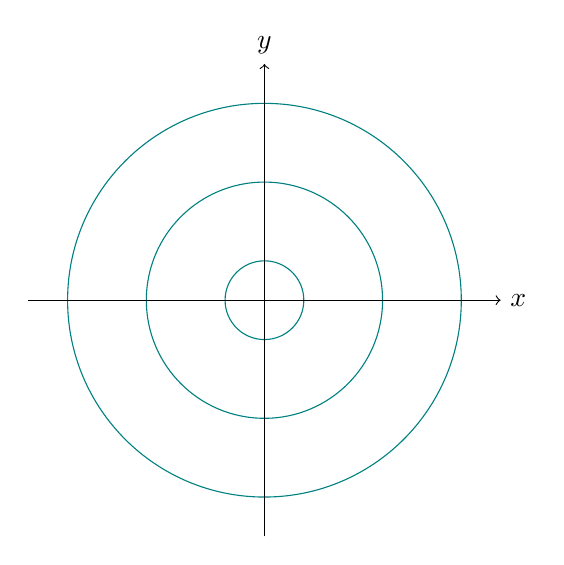
\begin{tikzpicture}[declare function={f(\x,\y)=\x*\x+\y*\y;}]
\def\xmax{2.5} \def\xmin{-2.5}
\def\ymax{2.5} \def\ymin{-2.5}


\draw[color=teal] (0,0) circle[radius=0.5];
%\draw[color=teal] (0,0) circle[radius=1];
\draw[color=teal] (0,0) circle[radius=1.5];
%\draw[color=teal] (0,0) circle[radius=2];
\draw[color=teal] (0,0) circle[radius=2.5];

\draw[->] (\xmin-.5,0)--(\xmax+.5,0) node[right] {$x$};
\draw[->] (0,\ymin-.5)--(0,\ymax+.5) node[above] {$y$};
\end{tikzpicture}
\end{document}